\section{Method}
\label{sec:method}

Auto MC-Reward consists of three components: Reward Designer, Reward Critic, and Trajectory Analyzer. Given the environment information and task descriptions, the Reward Designer proposes the reward function by coding an executable Python function with pre-defined observation inputs. The Reward Critic verifies if the proposed reward function is self-consistent and if it meets the format requirements. The designed reward function which passes the Reward Critic is used to train agents in the environment. To improve the designed reward function according to empirical experience, the Trajectory Analyzer is proposed to summarize possible failure causes and provide refinement suggestions on the reward function based on the inference trajectories of the trained agents. Then the Reward Designer modifies the reward function based on the feedback from Trajectory Analyzer. Figure~\ref{fig:pipeline} shows the overview of the Auto MC-Reward.


\subsection{Reward Designer}
\label{sec:designer}

We utilize a Reward Designer to generate the reward function code to provide intermediate instructive learning signals to the agent. It takes as input task descriptions, game information, and reward function requirements, generating reward functions in executable code form. When updating reward function, we also provide analysis of the agent's performance when interacting with the game environment. The input prompt is introduced in Section~\ref{sec:imple_detail}.

The generated reward function uses a pre-defined observation format as input. This includes the nearest distance of each block type within the visible range in the current and previous steps, changes in inventory between adjacent steps, health points, and the agent's location in each past step. These parameters can provide information on the agent's current and historical states, assisting the reward function in various situations.



\vspace{0.5em}\noindent\textbf{Multi-Step Memory}. Long-term tasks require the transfer of information across multiple steps. 
Thus, we introduce a multi-step memory mechanism. It is provided to Reward Designer as a empty dictionary at the beginning, and the reward function can save necessary data into the memory to be used in future steps.
In the actual reward function of the explore-tree task, we observed that the agent records the distance to a tree at each step, thereby encouraging getting closer with the tree than the previous step.

\vspace{0.5em}\noindent\textbf{Chain of Thought}. We require the LLM to first describe its design thoughts, such as considering potential failure reasons and the details of the reward function design. These thoughts are to be written as comments at the beginning of the code. This is a mechanism similar to Chain of Thought (CoT)~\cite{wei2022chain}, where the thought process precedes the coding implementation. In the specific code implementation, necessary comments will also be generated every few lines (\eg, ``Check if lava is in the field of view in the previous step''). This approach not only allows Reward Designer to refer to the text-form thoughts during reward function initialization, but also assists subsequent Reward Critic in assessing the code's rationality, and helps Reward Designer to understand the current reward function's purpose when updating the reward function. 


\vspace{0.5em}\noindent\textbf{Scale Constraints}. We impose a specific scale constraint for the reward function, where the LLM generates two sub-functions: dense and sparse. \emph{Sparse} denotes rewards for achieving the final goal or heavy penalties (like death), while \emph{dense} represents dense intermediate signals during the task completion process. We preset their numerical values and only allow the LLM to determine their positivity or negativity, limiting \emph{sparse} to $\{1, 0, -1\}$, and \emph{dense} to $\{0.1, 0, -0.1\}$. They are then added together for the final reward. Therefore, the final reward values can be one value of $\{\pm1.1, \pm1.0, \pm 0.9, \pm0.1, 0 \}$. The final reward is calculated as $R = \operatorname{sgn}(sparse) * 1 + \operatorname{sgn}(dense) * 0.1$, where $\operatorname{sgn}$ denotes the sign function.
This is to keep the reward within a reasonable range, allowing the LLM to focus on various scenarios that need to be considered in the reward function, rather than trivial tasks like adjusting the reward value.


\begin{figure}[!tb]
    \centering
    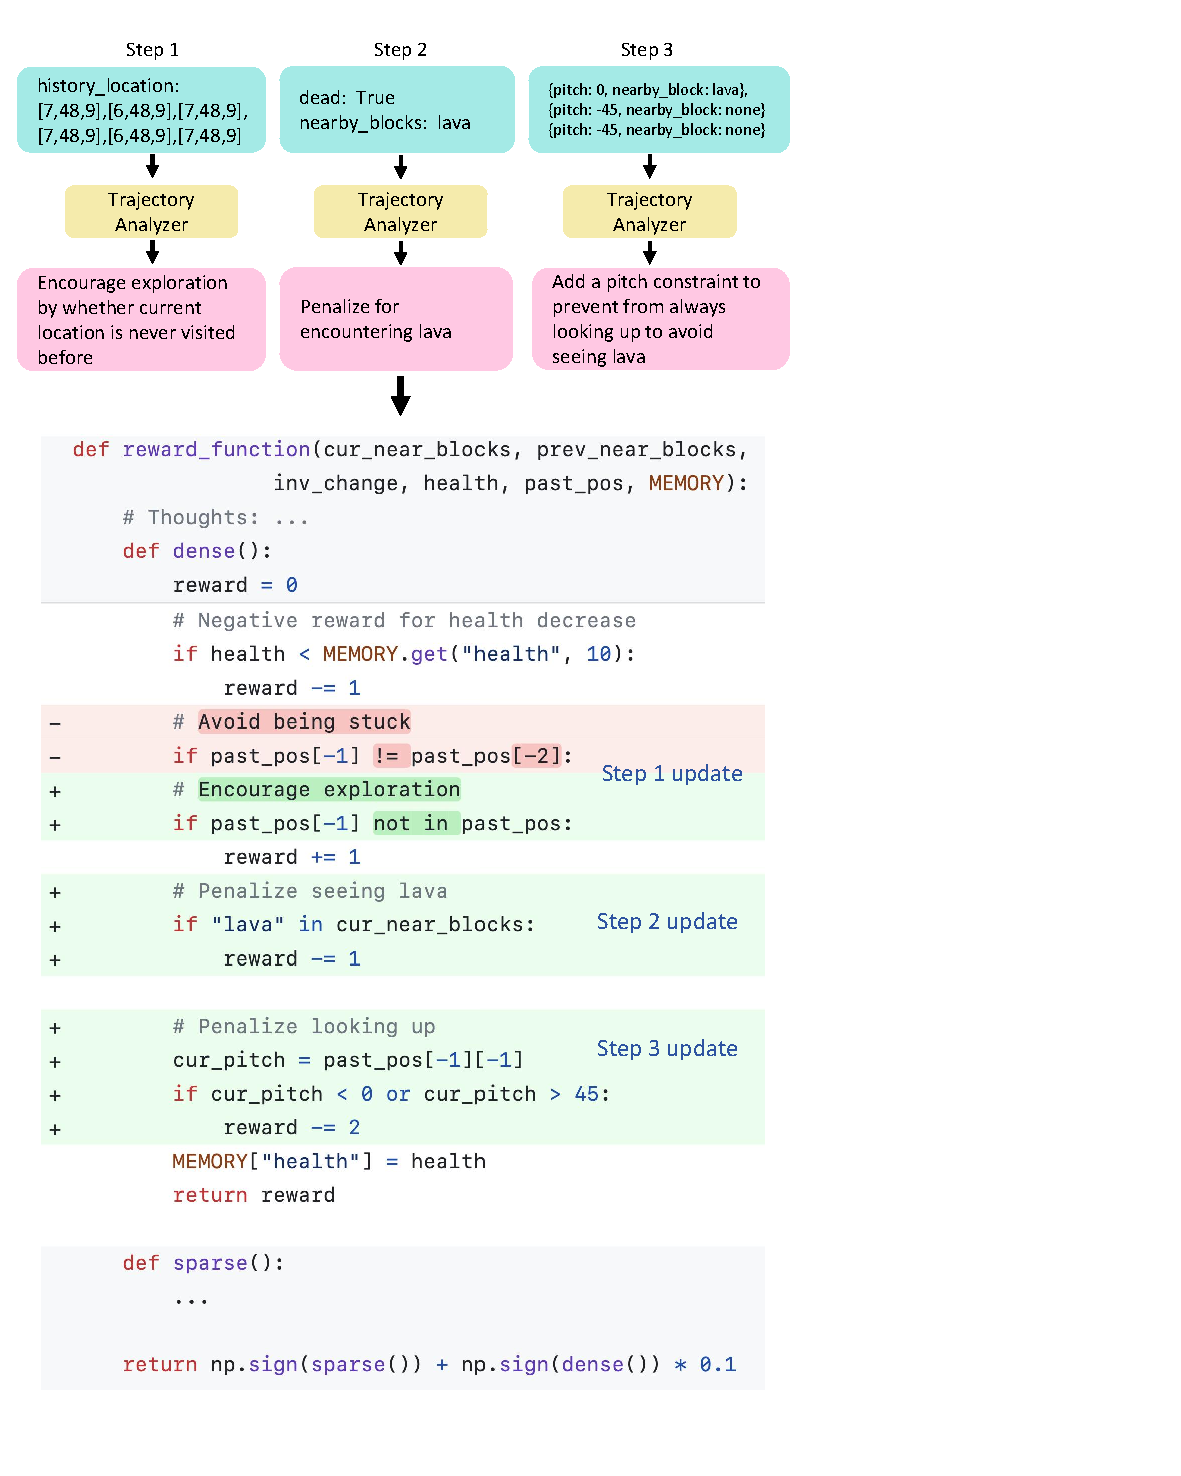
\includegraphics[width=0.43\textwidth]{figs/code_update8.pdf}
    \vspace{-5pt}
    \caption{Example of updating the reward function. Trajectory Analyzer provides analysis for three scenarios at different steps, and then Reward Designer update the reward function based on the suggestions. We only display part of the trajectory data for brevity. \textbf{Step 1}: rewrite the code of encouraging exploration to avoid going back and forth. \textbf{Step 2}: add lava penalty to avoid falling into lava. \textbf{Step 3}: add pitch constraint to avoid constantly looking up to avoid lava.}
    \label{fig:code}
    \vspace{-10pt}
\end{figure}



\subsection{Reward Critic}
In practice, it is difficult for LLM to generate a relatively complete reward function in the beginning. There may be errors in understanding parameter formats and data types (\textbf{syntax errors}), failure to consider game-specific information, or misunderstanding of tasks (\textbf{semantic errors}), etc. 

In order to eliminate above errors that are not easy to find, we design a LLM based Reward Critic to automatically review the designed reward function. In addition to checking for syntax errors, Reward Critic is also asked to check the quality of the reward function to further eliminate semantic errors. Specifically, we require Reward Critic to check whether the current code implementation matches its thoughts, whether it meets the reward function design requirements, and whether it takes game information into account. If the review fails, the Critic will provide a critique, and the Reward Designer will then modify the reward function based on the criterion and submit it for review again. The above process is repeated up to 3 times.

If an error occurs during the execution of the reward function in the process of interacting with the environment, the Python traceback of the error message will be fed back to Reward Designer for modification. These errors may include misunderstandings of input parameters, list index out of range, uninitialized keys in dictionaries, and other such issues. Some runtime errors only appear during the actual execution of the code.


\subsection{Trajectory Analyzer}\label{sec:trajectory_analyzer}
LLMs have the ability to understand environmental information and task instructions through in-context prompts to generate dense rewards. However, this zero-shot approach completely relies on LLM’s understanding of the task and imagination of the problems it may face, and it is difficult to ensure the effectiveness of the designed reward. Take the the yellow highlighted part in Figure~\ref{fig:pipeline} as an example, in the initially designed reward function, Reward Designer does not consider the situation where the agent would encounter lava and be burned to death. Thus, in order to introduce empirical improvements to the designed dense reward, we propose to use LLMs, named as Trajectory Analyzer, to summarize the historical information of the interaction between the trained agent and the environment and use it to guide the revision of the reward function. The division of labor of Reward Designer and Trajectory Analyzer allows for independent operations of data analysis and reward function updates. Trajectory Analyzer does not need to know the details of the reward function, and Reward Designer does not need to process complex trajectory data.

Specifically, the current trained model is used to interact with the environment and obtain $K$ trajectories.
Then, we truncate these trajectories and use a LLM to summarize the observations of the last consecutive $L$ frames of each failed trajectory to automatically infer its possible failure reasons. Based on the analysis of the reasons for the failure, the LLM Trajectory Analyzer is asked to propose key points that Reward Designer needs to consider in the next round of reward function revision. For instance, failure scenarios where punishment is not considered, misalignment of dense reward and sparse reward causes the agent's behavior to deviate from the final goal, etc.



Figure~\ref{fig:code} shows an example of multiple rounds of improving the reward function during the search for diamonds. In the first step, through analysis of the trajectory, Trajectory Analyzer finds that the agent would opportunistically find a shortcut to increase the reward, that is, move back and forth to deceive the reward function into thinking that the agent is moving actively. Therefore, the Reward Designer modifies the code snippet that encourages the agent to move, \emph{i.e.} encourage the agent to appear in unvisited locations as much as possible. Although the initially designed reward function has taken into account the penalty for the loss of the agent's health, the agent still cannot effectively learn to avoid lava.
When modifying the reward function in the second round, Trajectory Analyzer discovers through the failed trajectory that the agent may die from lava, so it is suggested that Reward Designer increase the penalty for encountering lava, as shown in the step 2 update in Figure \ref{fig:code}.
According to the interactive experience, Reward Designer explicitly punishes the continuous appearance of lava in the field of view. However, the excessive punishment of lava caused the agent to choose to turn its perspective upward or downward to avoid the appearance of lava in the visible range, making it impossible for the agent to continue effective exploration, which deviates from the ultimate goal. To this end, Reward Designer further constrain the agent's perspective in step 3, so that the lava disappeared from the agent's perspective by turning left/right while continuing to search for diamonds, which is the desired strategy. Figure~\ref{fig:lava_cow}(a) shows the successful trajectory of avoiding lava: 
The agent sees the lava after breaking the stone ahead using iron pickaxe, and then turn left to avoid the lava through the mining tunnel.


\begin{algorithm}[!tb]
\footnotesize
    \caption{\small{Auto MC-Reward Training Pseudo Code}}
    \label{alg}
    \begin{algorithmic}
        \REQUIRE Task ($T$), Inital Agent ($A_0$), Environment (Env), Max  number of Critic reviews ($N_\text{Critic}$)
        \ENSURE Final Agent ($A_N$), Final Reward ($R_N$)
        \STATE Summary = None
        \STATE Critique = None
        \STATE $R_0$ = None
        \FOR{$i = 1, \dots, N$}
            \STATE R$_i$ = RewardDesigner(Summary, Critique, $T$, $R_{i-1}$)
            \FOR{$j = 1, \dots, N_\text{Critic}$}
                \STATE Critique, Done = RewardCritic($R_i$)
                \IF{Done}
                    \STATE break
                \ELSE
                    \STATE $R_i$ = RewardDesigner(Summary, Critique, $T$, $R_{i}$)
                \ENDIF
            \ENDFOR
            \STATE $A_i$ = TrainAgent($A_0$, $R_{i}$, Env, $T$)
            \STATE Traj$_i$, Stat$_i$ = Eval(Env, $A_i$)
            \STATE Summary = TrajectoryAnalyzer(Traj$_i$, Stat$_i$)
            \STATE Critique = None
        \ENDFOR
    \end{algorithmic}
    \label{alg:pseudo}
\end{algorithm}





